%% LaTeX2e class for student theses
%% sections/content.tex
%%
%% Karlsruhe University of Applied Sciences
%% Faculty of  Computer Science and Business Information Systems
%% Distributed Systems (vsys)
%%
%% Prof. Dr. Christian Zirpins
%% christian.zirpins@hs-karlsruhe.de
%%
%%
%% Version 0.2, 2017-11-15
%%
%% --------------------------------------------------------
%% | Derived from sdqthesis by Erik Burger burger@kit.edu |
%% --------------------------------------------------------

\chapter{Implementierung eines ActivityPub Prototyps}
Die IDataSource Implementierung wird für das Unternehmen angefertigt in der die Bachelor Thesis bearbeitet wird. Im Falle man möchte den Service mit einer anderen Datenquelle versorgen, kann das IDataSource Interface implementiert und so angepasst werden, dass eine andere Datenbank Verwendung findet.\\
\begin{figure}[h]
	\begin{minipage}{\textwidth}
		\centering
		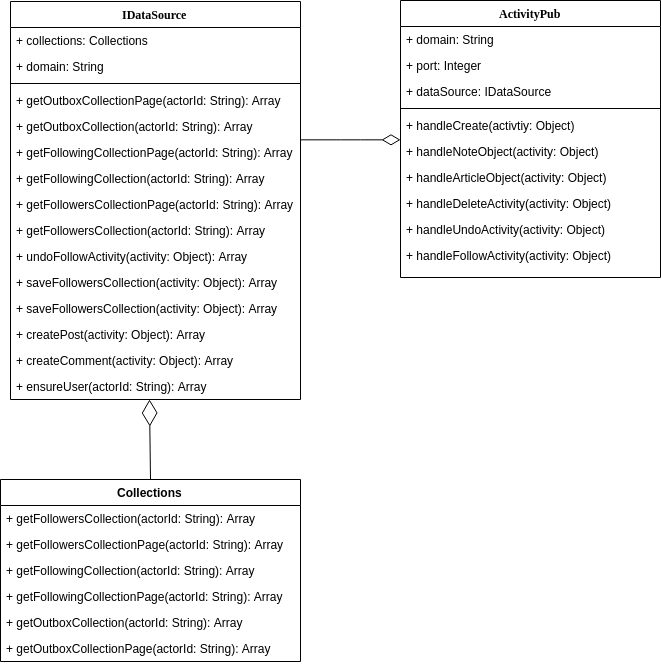
\includegraphics[scale=0.6]{figures/klassendiagramm-activitypub.png}
		\label{klassendiagramm-activitypub}
		\caption{Hauptkomponenten des förderierten Servers}
	\end{minipage}
\end{figure}
Obig abgebildetes Klassendiagramm zeigt die Hauptkomponenten des ActivityPub Services und die enthaltenen Methoden.\\
In der Collections Klasse sind Weiterleitungen zu entsprechenden Methoden der Datenquelle; Sie dient ausschließlich der Lesbarkeit für den Entwickler.\\
Bei der ActivityPub Klasse handelt es sich um den Eingangspunkt. Die entsprechenden Anfrage-Handler wandeln die Anfrage in einen Service Aufruf um. Diese Klasse enthält nicht nur Handler für eingehende, sondern auch Methoden zum senden von Anfragen.\\

Um eine möglichst Modulare Implementierung zu gewährleisten wurden alle Datenbankspezifischen Methoden in das IDataSource Interface ausgelagert. Durch die Implementierung dieses Interfaces können Aktivitäten ActivityPub konform empfangen werden. Das senden wiederum muss jedes Backend selbst implementieren. Dafür stehen in der ActivityPub Klasse Methoden zum senden von Aktivitäten bereit. Durch einfaches importieren der ActivityPub Klasse erhält man eine Instanz. Darüber sind die Methoden verfügbar.\\

Es ist auch möglich andere Datenquellen als die in der Bachelor Arbeit verwendete GraphQL Schnittstelle zu nutzen, wie z. B. MySQL oder MongoDB.\\

Getestet wird die Implementierung mit dem Cucumber Test-Framework, welches ein Werkzeug zum ausüben von \gls{bdd} ist. Die Tests selbst werden im Rahmen von Cucumber als sogenannte \glqq Feature\grqq's bezeichnet und haben die Dateiendung \glqq .feature\grqq. Geschrieben sind die Tests in der Gherkin Sprache welche eine Sammlung von Syntax ist um diese auf entsprechende Aktionen, sogenannte \glqq Steps\grqq~abzubilden. Es wurden bei der Gherkin Syntax extra leicht verständliche Schlüsselworte gewählt um die Tests auch für Benutzer, Produktbesitzer und weitere lesbar zu halten. Somit muss nur die Gherkin Sprache bekannt sein um die Features schreiben zu können. Das Verständnis beim lesen ergibt sich aus der Verwendung natürlicher Sprachkonstrukte als Schlüsselwörter.\\

Unter \gls{tdd} versteht man eine Vorgehensweise beim Entwickeln von Software. Dabei werden zuerst fehlschlagende Tests geschrieben, um diese im zweiten Schritt durch eine Implementierung der Komponenten zur erfolgreichen Ausführung zu bringen. Im dritten Schritt werden die Tests angepasst und der Zyklus wiederholt sich.\\

Bei der Softwareentwicklung mit dem \gls{bdd} Ansatz wird im Grunde genommen Wert auf eine hohe Kommunikation zwischen allen beteiligten im Entwicklungsprozess gelegt. Werkzeuge wie Cucumber fördern dabei die Lesbarkeit von Softwaretests und somit auch die Kommunikation zwischen Programmierern und dem Rest des Teams. Zudem ist es für Neueinsteiger leichter einen Überblick über die Funktionalität des Systems zu bekommen\footnote{Vlg. Cucumber Gemeinschaft, Absatz 1}.\\
 
\section{Server-zu-Server Protokoll}
Es wird eine Teilmenge der ActivityPub Funktionalität implementiert, die angepasst ist auf die Anforderungen der Firma in welcher diese Arbeit angefertigt wird. Dabei handelt es sich um folgende Aktivitäten des Standards: \textit{Create}, \textit{Update}, \textit{Delete}, \textit{Follow}, \textit{Undo}, \textit{Accept}, \textit{Reject}, \textit{Like}, \textit{Dislike}.\\

Die ersten drei Aktivitäten werden zum Manipulieren von Objekten wie z. B. einem Artikel benötigt. \textit{Follow} und \textit{Undo} sind zum folgen eines Nutzers so wie zum rückgängig machen verschiedener Aktivitäten. Wenn einem Nutzer gefolgt wurde, wird eine \textit{Accept} Aktivität an die \textit{Inbox} des Folgenden gesendet mit der \textit{Follow} Aktivität als Objekt.\\

Der Funktionsumfang des förderierten Servers beschränkt sich auf den folgenden:
\begin{itemize}
	\item Empfangen von \textit{\textbf{Article}} und \textit{\textbf{Note}} Objekten am Geteilten Nachrichteneingang (sharedInbox, Inbox)
	\item Empfangen von \textit{\textbf{Like}} und \textit{\textbf{Follow}} Aktivitäten am Geteilten Nachrichteneingang
	\item Empfangen von \textit{\textbf{Undo}} und \textit{\textbf{Delete}} Aktivitäten für \textit{\textbf{Articles}} und \textit{\textbf{Notes}} am Geteilten Nachrichteneingang 
	\item Bereitstellen eines \textit{\textbf{Webfinger}} und \textit{\textbf{Aktoren}} Objektes
	\item Bereitstellen der \textit{\textbf{Followers}}, \textit{\textbf{Following}} und \textit{\textbf{Outbox}} Sammlungen
\end{itemize}

Artikel und Notizen werden bei der in dieser Arbeit angefertigten Implementierung gleich behandelt. Beim empfangen einer Create Aktivität die eine Notiz oder Artikel als Objekt Attribut hat, wird der Artikel über die IDataSource Implementierung erstellt und entsprechende Metadaten zum rekonstruieren der ID's gespeichert. Somit können empfangene \glqq Posts\grqq, welche an die Öffentlichkeit gerichtet sind, im Netzwerk angezeigt werden. Die Logik zum Empfangen von \glqq Posts\grqq~die an einzelne Nutzer gerichtet sind ist noch nicht vorhanden.\\

Eingehende HTTP POST Anfragen werden auf eine vorhandene Signatur Kopfzeile geprüft. Wird diese nicht gefunden, wird die Anfrage verworfen. Ist sie vorhanden, wird die Signatur geprüft indem das Aktoren Objekt über die zugehörige \textit{keyId} angefragt wird und die Signatur gegen den öffentlichen Schlüssel geprüft wird. Dies stellt sicher, das die Inhalte der Nachricht beim Transport nicht verändert wurde und zudem das die Aktivität von dem Nutzer stammt, der den passenden privaten Schlüssel besitzt. Eine Signatur bei der Übertragung von Servern untereinander wird demnach verwendet um die Authentizität der Daten überprüfen zu können.\\
